\section{Task2: Processing of our own $3$ scenarios of the accelerate methods}

We can implement the accelerate methods(NGP, TensoRF) on $3$ scenarios, which were introduced in \ref{scenarios}.

With the dataloader \ref{data loader}, we can use our own scenarios to run the accelerate methods and test the behaviors.

The vanilla NeRF without any acceleration \cite{nerf_pytorch} were also implemented as the baseline to compare with.

% --------------------------------
\subsection{basic settings}
\label{basic settings}

All the code were run under the environment of python3.10.

For the training mode of vanilla-NeRF and TensoRF, we choose the blender mode, and modify the correspondence dataloader.

Since our dataset is somehow bigger than the default once, so the scale should be modify by timing $4$, i.e. the parameter '\textit{aabb\_scale}' is set to be $4$, the '\textit{scene\_box}' is modifed from $[-1.5,-1.5,-1.5],[1.5,1.5,1.5]$ to $[-6,-6,-6],[6,6,6]$.

The training iterations for the vanilla NeRF, TensoRF, NGP, and the improvement method are all set to be default iterations. 

And other settings are by default.

% --------------------------------
\subsection{way to run the code}
\label{way to run code}

To run the code and see the results, the details are in the jupyter notebook \textit{NeRF.ipynb}, just run all modules in it would work. The running records are all in \textit{NeRF.ipynb}.

% --------------------------------
\subsection{results}
\begin{figure*}
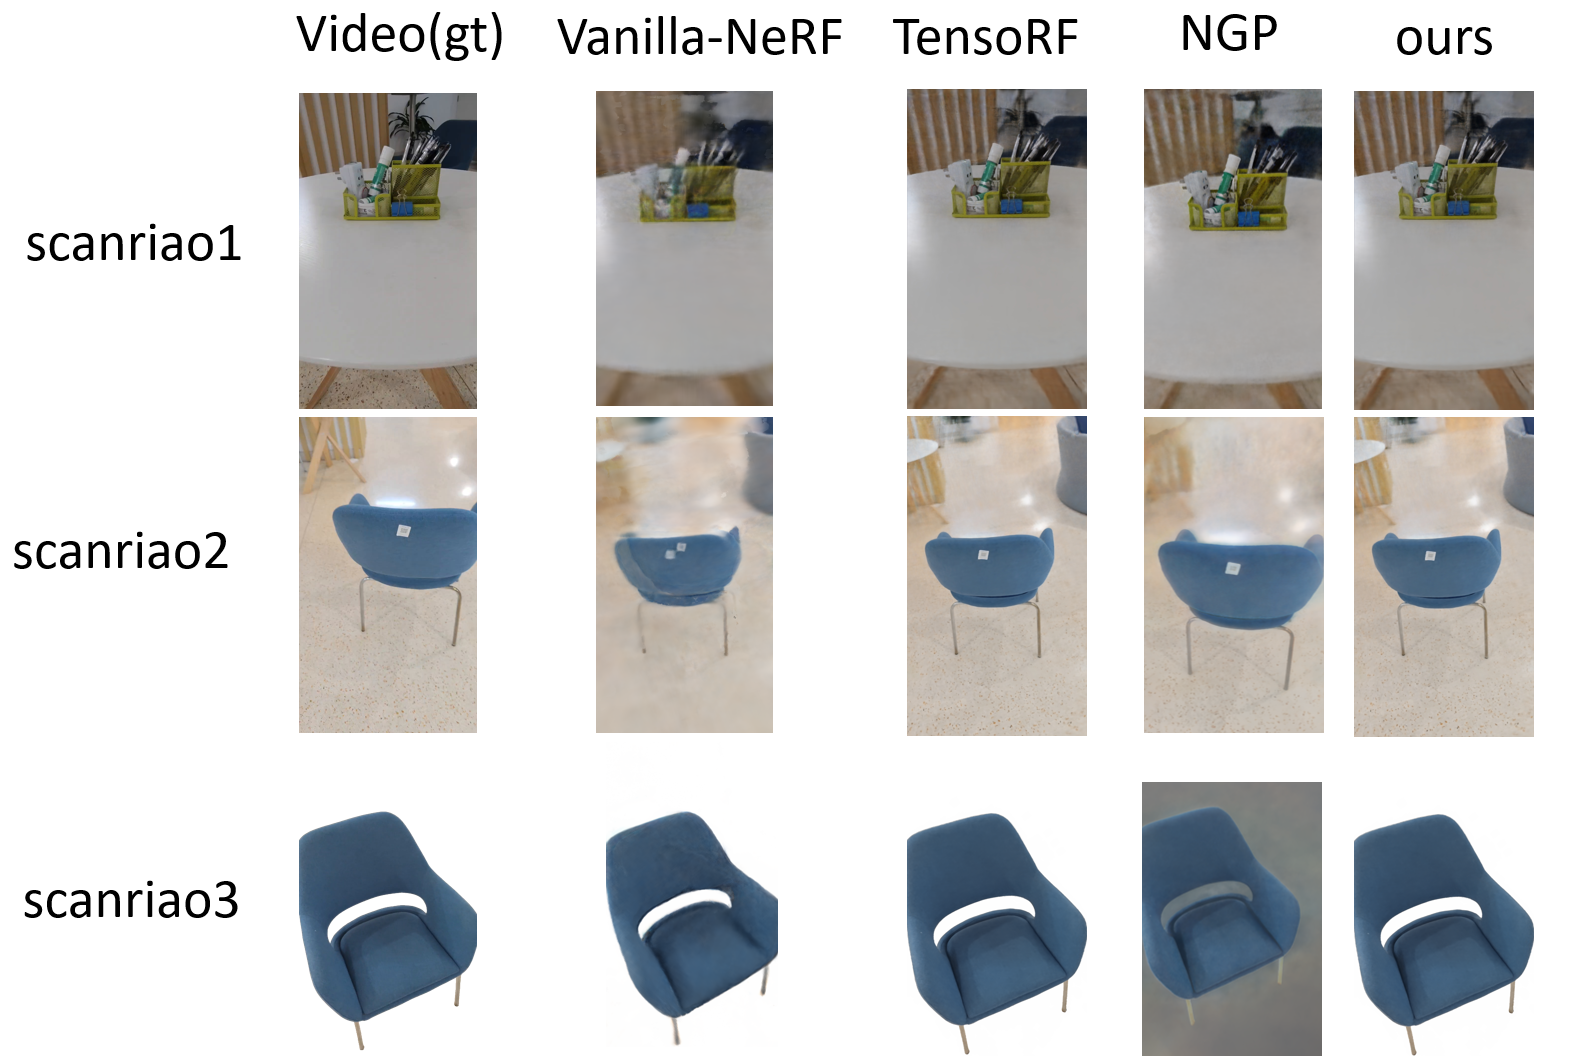
\includegraphics[width=0.9\textwidth]{result/result.png} 
\caption{novel synthesis view of the $3$ scenarios}
\label{result}
\end{figure*}

The running records are all in \textit{NeRF.ipynb}.

The metrics mentioned in \ref{metric} would be shown in section \ref{conclusion}. And the figures \ref{result} are one of the results of the novel synthesis view of the $3$ scenarios.

Since the dataset are seperated into training, testing, validation dataset. So all the novel synthesis view of the $3$ scenarios are chosen from the testing dataset, so the novel view exist ground truth for comparison.